% THIS DOCUMENT IS TAILORED TO REQUIREMENTS FOR SCIENTIFIC COMPUTING.  IT SHOULDN'T
% BE USED FOR NON-SCIENTIFIC COMPUTING PROJECTS
\documentclass[12pt]{article}

\usepackage{amsmath, mathtools}
\usepackage{amsfonts}
\usepackage{amssymb}
\usepackage{graphicx}
\usepackage{colortbl}
\usepackage{xr}
\usepackage{hyperref}
\usepackage{longtable}
\usepackage{xfrac}
\usepackage{tabularx}
\usepackage{float}
\usepackage{siunitx}
\usepackage{booktabs}
\usepackage{caption}
\usepackage{pdflscape}
\usepackage{afterpage}
\usepackage{svg}

\usepackage[round]{natbib}

%\usepackage{refcheck}

\hypersetup{
    bookmarks=true,         % show bookmarks bar?
    colorlinks=true,       % false: boxed links; true: colored links
    linkcolor=red,          % color of internal links (change box color with linkbordercolor)
    citecolor=green,        % color of links to bibliography
    filecolor=magenta,      % color of file links
    urlcolor=cyan           % color of external links
}

%% Comments

\usepackage{color}

\newif\ifcomments\commentstrue %displays comments
%\newif\ifcomments\commentsfalse %so that comments do not display

\ifcomments
\newcommand{\authornote}[3]{\textcolor{#1}{[#3 ---#2]}}
\newcommand{\todo}[1]{\textcolor{red}{[TODO: #1]}}
\else
\newcommand{\authornote}[3]{}
\newcommand{\todo}[1]{}
\fi

\newcommand{\wss}[1]{\authornote{blue}{SS}{#1}} 
\newcommand{\plt}[1]{\authornote{magenta}{TPLT}{#1}} %For explanation of the template
\newcommand{\an}[1]{\authornote{cyan}{Author}{#1}}

%% Common Parts

\newcommand{\progname}{2D-RAPP} % PUT YOUR PROGRAM NAME HERE
\newcommand{\authname}{Ziyang(Ryan) Fang} % AUTHOR NAMES                  

\usepackage{hyperref}
    \hypersetup{colorlinks=true, linkcolor=blue, citecolor=blue, filecolor=blue,
                urlcolor=blue, unicode=false}
    \urlstyle{same}
                                


% For easy change of table widths
\newcommand{\colZwidth}{1.0\textwidth}
\newcommand{\colAwidth}{0.13\textwidth}
\newcommand{\colBwidth}{0.82\textwidth}
\newcommand{\colCwidth}{0.1\textwidth}
\newcommand{\colDwidth}{0.05\textwidth}
\newcommand{\colEwidth}{0.8\textwidth}
\newcommand{\colFwidth}{0.17\textwidth}
\newcommand{\colGwidth}{0.5\textwidth}
\newcommand{\colHwidth}{0.28\textwidth}

% Used so that cross-references have a meaningful prefix
\newcounter{defnum} %Definition Number
\newcommand{\dthedefnum}{GD\thedefnum}
\newcommand{\dref}[1]{GD\ref{#1}}
\newcounter{datadefnum} %Datadefinition Number
\newcommand{\ddthedatadefnum}{DD\thedatadefnum}
\newcommand{\ddref}[1]{DD\ref{#1}}
\newcounter{theorynum} %Theory Number
\newcommand{\tthetheorynum}{TM\thetheorynum}
\newcommand{\tref}[1]{TM\ref{#1}}
\newcounter{tablenum} %Table Number
\newcommand{\tbthetablenum}{TB\thetablenum}
\newcommand{\tbref}[1]{TB\ref{#1}}
\newcounter{assumpnum} %Assumption Number
\newcommand{\atheassumpnum}{A\theassumpnum}
\newcommand{\aref}[1]{A\ref{#1}}
\newcounter{goalnum} %Goal Number
\newcommand{\gthegoalnum}{GS\thegoalnum}
\newcommand{\gsref}[1]{GS\ref{#1}}
\newcounter{instnum} %Instance Number
\newcommand{\itheinstnum}{IM\theinstnum}
\newcommand{\iref}[1]{IM\ref{#1}}
\newcounter{reqnum} %Requirement Number
\newcommand{\rthereqnum}{R\thereqnum}
\newcommand{\rref}[1]{R\ref{#1}}
\newcounter{nfrnum} %NFR Number
\newcommand{\rthenfrnum}{NFR\thenfrnum}
\newcommand{\nfrref}[1]{NFR\ref{#1}}
\newcounter{lcnum} %Likely change number
\newcommand{\lthelcnum}{LC\thelcnum}
\newcommand{\lcref}[1]{LC\ref{#1}}

\usepackage{fullpage}

\newcommand{\deftheory}[9][Not Applicable]
{
\newpage
\noindent \rule{\textwidth}{0.5mm}

\paragraph{RefName: } \textbf{#2} \phantomsection 
\label{#2}

\paragraph{Label:} #3

\noindent \rule{\textwidth}{0.5mm}

\paragraph{Equation:}

#4

\paragraph{Description:}

#5

\paragraph{Notes:}

#6

\paragraph{Source:}

#7

\paragraph{Ref.\ By:}

#8

\paragraph{Preconditions for \hyperref[#2]{#2}:}
\label{#2_precond}

#9

\paragraph{Derivation for \hyperref[#2]{#2}:}
\label{#2_deriv}

#1

\noindent \rule{\textwidth}{0.5mm}

}

\begin{document}

\title{Software Requirements Specification for 2D Robot Arms for Path Planning} 
\author{\ Ziyang(Ryan) Fang}
\date{\today}
	
\maketitle

~\newpage

\pagenumbering{roman}

\tableofcontents

~\newpage

\section*{Revision History}

\begin{tabularx}{\textwidth}{p{3cm}p{2cm}X}
\toprule {\bf Date} & {\bf Version} & {\bf Notes}\\
\midrule
Feb 02 2025 & 1.0 & Notes\\
% Date 2 & 1.1 & Notes\\
\bottomrule
\end{tabularx}



~\newpage

\section{Reference Material}

This section records information for easy reference.

\subsection{Table of Units}

Throughout this document SI (Syst\`{e}me International d'Unit\'{e}s) is employed
as the unit system.  In addition to the basic units, several derived units are
used as described below.  For each unit, the symbol is given followed by a
description of the unit and the SI name.
~\newline

\renewcommand{\arraystretch}{1.2}
  \noindent \begin{tabular}{l l l} 
    \toprule		
    \textbf{symbol} & \textbf{unit} & \textbf{SI}\\
    \midrule 
    \si{\milli\metre} & length & millimetre \\
    % \si{\kilogram} & mass & kilogram \\
    \si{\second} & time & second \\
    \( q \) & joint angle & radians \\
    \(\dot{q}\) & joint velocity & rad/s \\
    \(\ddot{q}\) & joint acceleration & rad/s\(^2\)  \\
    % \si{\newton\metre} & torque & newton metre \\
    \bottomrule
  \end{tabular}
  %	\caption{Provide a caption}
%\end{table}



\subsection{Table of Symbols}

The following table provides a summary of the symbols used throughout this document, along with their respective units and descriptions. The choice of symbols aligns with conventions in robotics and motion planning literature to ensure consistency and clarity. Symbols are listed in alphabetical order for easy reference.

\renewcommand{\arraystretch}{1.2}
%\noindent \begin{tabularx}{1.0\textwidth}{l l X}
\noindent \begin{longtable*}{l l p{12cm}} \toprule
\textbf{symbol} & \textbf{unit} & \textbf{description}\\
\midrule 
\( L \) & \si{\milli\metre} & Link length of the robot arm \\
\( q \) & radians & Joint angle \\
\( \dot{q} \) & rad/s & Joint angular velocity \\
\( \ddot{q} \) & rad/s\(^2\)  & Joint angular acceleration \\
\( x, y \) & \si{\milli\metre} & Cartesian coordinates of the end-effector \\
\( T \) & \si{\second} & Total time for motion execution \\
\( t \) & \si{\second} & Time step \\
\( \mathbf{q}_{\text{init}} \) & radians & Initial joint configuration \\
\( \mathbf{q}_{\text{goal}} \) & radians & Goal joint configuration \\
\( O_i \) & \si{\milli\metre} & Position of the \(i\)-th obstacle (circular) \\
\( r_i \) & \si{\milli\metre} & Radius of the \(i\)-th obstacle \\
% \( M \) & - & Number of discrete joint positions in A* search grid \\
\( \theta_i \) & radians & Discretized joint angle for A* search \\
% \( \mathcal{G} \) & - & Occupancy grid (joint space) \\
\( \mathbf{p}_i \) & \si{\milli\metre} & Position of the \(i\)-th joint \\

\bottomrule
\end{longtable*}


\subsection{Abbreviations and Acronyms}

\renewcommand{\arraystretch}{1.2}
\begin{tabular}{l l} 
  \toprule		
  \textbf{symbol} & \textbf{description}\\
  \midrule 
  A & Assumption\\
  DD & Data Definition\\
  GD & General Definition\\
  GS & Goal Statement\\
  IM & Instance Model\\
  LC & Likely Change\\
  PS & Physical System Description\\
  R & Requirement\\
  SRS & Software Requirements Specification\\
  TM & Theoretical Model\\
  IK & Inverse Kinematics \\
  FK & Forward Kinematics \\
  A* & A-star Pathfinding Algorithm \\
  DOF & Degrees of Freedom \\
  EE & End-Effector \\
  % \progname{} & 2DPL\\
  TM & Theoretical Model\\
  2D-RAPP & 2D Robot Arm Path Planning\\
  \bottomrule
\end{tabular}\\





\section{Introduction}
Path planning for robotic manipulators is a fundamental problem in robotics, enabling robots to move efficiently and safely within constrained environments. Unlike mobile robots that navigate in free space, robotic arms must operate in a higher-dimensional joint space, where each degree of freedom contributes to the overall complexity of motion planning. Traditional inverse kinematics (IK) methods solve for joint angles that satisfy end-effector goals, but they often struggle with obstacle avoidance and computational efficiency in real-time applications.

This document provides an overview of the Software Requirements Specification (SRS) for a 2D robotic arm path planning system based on a graph-based inverse kinematics (IK) approach with A* search. The developed program will be referred to as 2D Robot Arm Path Planning (2D-RAPP) throughout this document. This section explains the purpose of this document, the scope of the requirements, the characteristics of the intended reader, and the organization of the document.

\subsection{Purpose of Document}
The primary purpose of this document is to record the requirements of 2D-RAPP. Goals, assumptions, theoretical models, definitions, and other derivation information are specified, allowing the reader to fully understand and verify the purpose and scientific basis of 2D-RAPP. With the exception of system constraints, this SRS remains abstract, describing what problem is being solved, but not how to solve it.

This document serves as a starting point for subsequent development phases, including writing the design specification and the software verification and validation plan. The design document will show how the requirements are to be realized, including decisions on numerical algorithms, data structures, and programming frameworks. The verification and validation plan will outline the steps required to increase confidence in the software’s correctness, reliability, and performance. 

Although this SRS follows a structured documentation approach, it does not impose any specific software development methodology. Regardless of whether a waterfall, agile, or iterative development process is followed, it remains useful to present the documentation in a way that maintains clarity and logical structure, as recommended by Parnas and Clements.



\subsection{Scope of Requirements} 
The scope of the requirements includes path planning for a 2D robotic arm with N revolute joints, operating in a workspace with circular obstacles. The system is designed to compute collision-free paths in joint space, using distance-based inverse kinematics and search algorithms.


\subsection{Characteristics of Intended Reader} \label{sec_IntendedReader}
Reviewers of this documentation should have a fundamental understanding of robotics kinematics at an undergraduate level, specifically covering forward kinematics, inverse kinematics, and path planning. Familiarity with graph-based search algorithms (such as A*) and numerical optimization techniques is also recommended.

The users of 2D-RAPP (e.g., robotics researchers, engineers) may have varying levels of expertise, as explained in Section~\ref{SecUserCharacteristics}. However, those involved in reviewing, modifying, or maintaining this SRS should have a strong background in computational kinematics and algorithmic path planning.


\subsection{Organization of Document}

This document follows the standard structure of an SRS for scientific computing software. It begins with the problem statement and goals, followed by theoretical foundations, definitions, and assumptions. The document then presents instance models and specific requirements.

The problem is introduced through kinematic models and path planning techniques, including forward and inverse kinematics and graph-based search methods. Assumptions related to joint constraints and obstacle avoidance are also outlined.

Readers can approach this document either top-down, starting from goals to implementation, or bottom-up, beginning with instance models and tracing back to theoretical foundations. The instance model IM:PathPlanning defines the core algorithm for collision-free motion planning of a 2D robot arm.


\section{General System Description}

This section provides general information about the system.  It identifies the
interfaces between the system and its environment, describes the user
characteristics and lists the system constraints. 


\subsection{System Context}


Fig.~\ref{Fig:SysCon} illustrates the system context. The circle represents the user, an external entity providing inputs to the system. The rectangle represents the software system, 2D-RAPP. Arrows indicate the data flow between the user and the system.

\begin{figure}[h!]
\centering
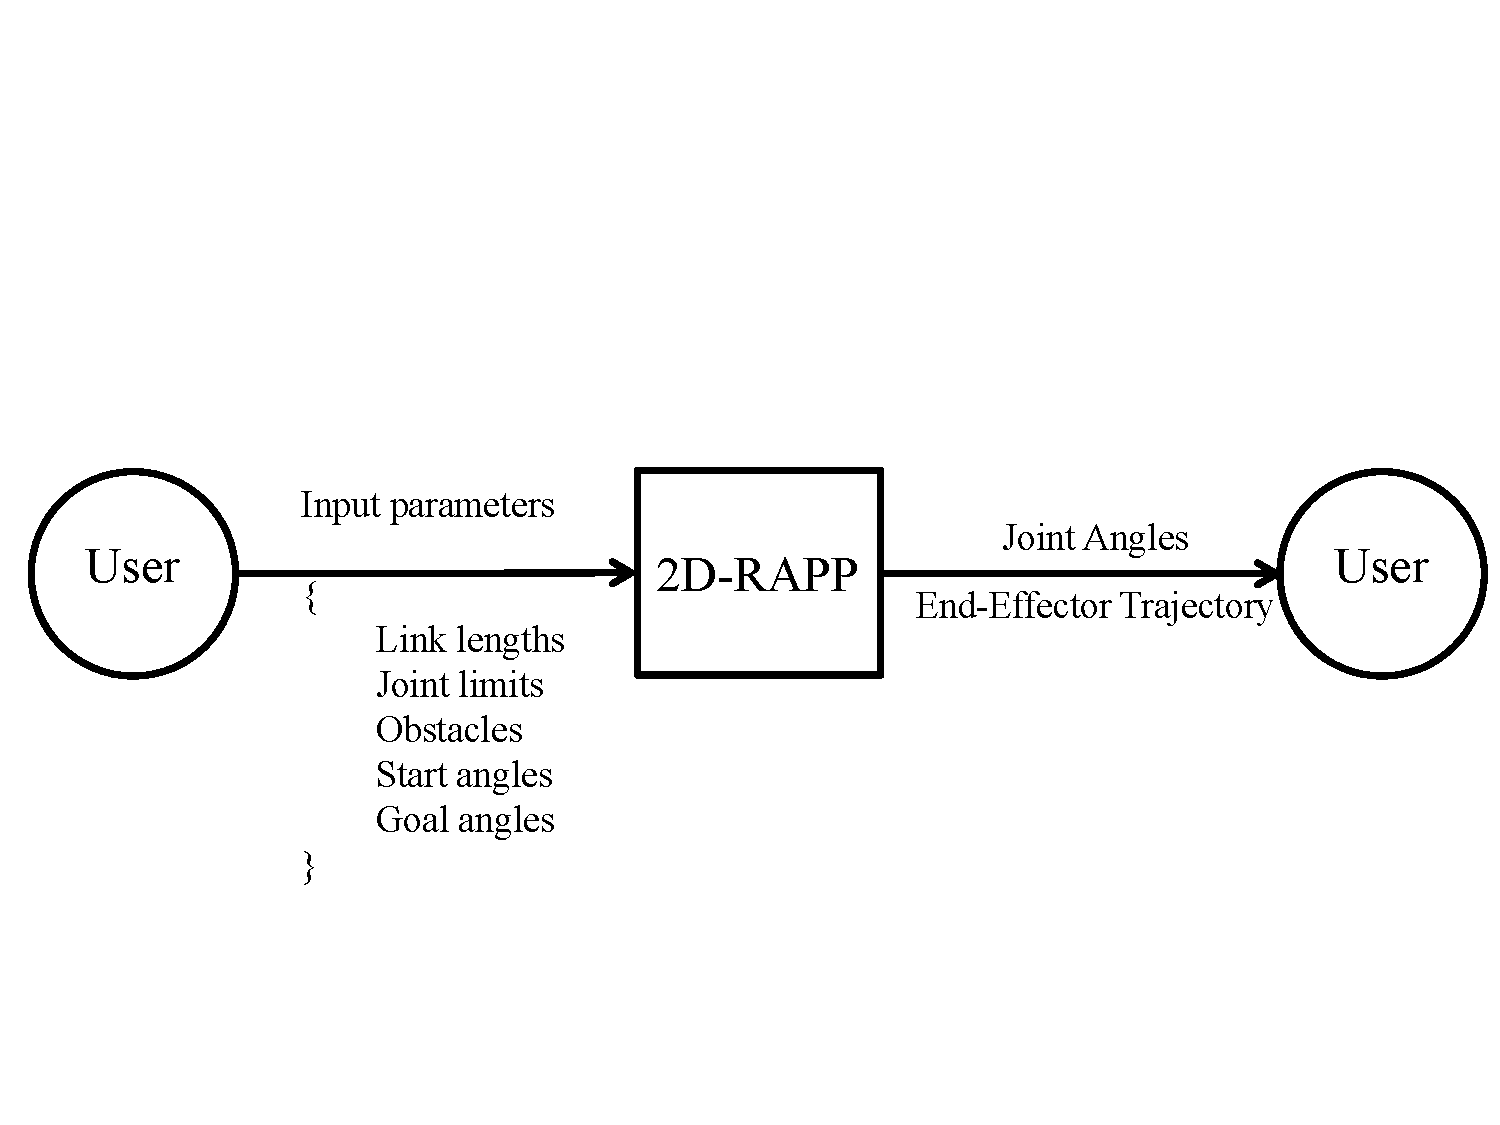
\includegraphics[width=0.8\textwidth]{SystemContextFigure}
\caption{System Context}
\label{Fig:SysCon}
\end{figure}

The interaction between the user and the system is described as follows:

\subsubsection*{User Responsibilities}
\begin{itemize}
    \item Provide the input data to the system, including:
    \begin{itemize}
        \item Initial joint angles (\(q_{\text{init}}\)) to specify the starting configuration of the robotic arm.
        \item Goal position (\(x_{\text{goal}}, y_{\text{goal}}\)) to indicate the desired end-effector target.
        \item Obstacle data, including radii (\(r_i\)) and positions (\(O_i = (x_i, y_i)\)).
    \end{itemize}
    \item Ensure the input data is accurate and in the required units.
\end{itemize}

\subsubsection*{2D-RAPP Responsibilities}
\begin{itemize}
    \item Detect input errors, such as invalid data types or inconsistent units.
    \item Verify that the inputs satisfy physical and software constraints.
    \item Compute a collision-free trajectory for the robotic arm, including:
    \begin{itemize}
        \item Joint angles (\(q\), \(\dot{q}\), \(\ddot{q}\)) for each motion stage.
        \item Cartesian path (\(x, y\)) of the end-effector.
    \end{itemize}
    \item Provide a visual representation of the robotic arm's movement and obstacle avoidance.
    \item Detect unreachable goal positions:
    \begin{itemize}
        \item If the target position is not reachable due to kinematic limitations or obstacles, return an empty result.
        \item Notify the user that the goal position cannot be reached.
    \end{itemize}
\end{itemize}

This system context defines the roles and interactions between the user and the 2D-RAPP system, ensuring clarity in the data flow and system responsibilities.


\subsection{User Characteristics} \label{SecUserCharacteristics}
The intended users of \progname{} are individuals with a background in robotics, computer science, and mechanical engineering. They are expected to have a fundamental understanding of kinematics, particularly inverse kinematics, and be familiar with basic path planning algorithms. 


\subsection{System Constraints}
There are no system constraints.


\section{Specific System Description}

This section first presents the problem description, which gives a high-level
view of the problem to be solved.  This is followed by the solution characteristics
specification, which presents the assumptions, theories, definitions and finally
the instance models. The system focuses on generating a collision-free trajectory for a 2D robotic arm in an environment with static obstacles. The robotic arm is modeled as a serial manipulator with revolute joints, and its configuration is defined by a set of joint angles.


\subsection{Problem Description} \label{Sec_pd}

\progname{} is intended to solve the path planning for 2D robotic arms.



\subsubsection{Terminology and  Definitions}


This subsection provides a list of terms that are used in the subsequent
sections and their meaning, with the purpose of reducing ambiguity and making it
easier to correctly understand the requirements:

\begin{itemize}

  \item \textbf{Joint space:} The space defined by the possible values of the robot arm’s joint angles.
  
  \item \textbf{Workspace:} The Cartesian space where the end-effector of the robotic arm can reach.
  
  \item \textbf{Obstacle:} A static circular object in the workspace that the robotic arm must avoid.
  
  \item \textbf{Trajectory:} A sequence of joint configurations representing a smooth motion of the robotic arm from the start to the goal.
  
  \item \textbf{Configuration:} A specific set of joint angles that fully describes the position of the robotic arm.
  
  \item \textbf{Collision detection:} The process of determining whether the robotic arm intersects with an obstacle.
  
  \item \textbf{Path planning:} The process of computing a collision-free sequence of configurations to move the robotic arm from the start to the goal.
  
  \item \textbf{Inverse kinematics:} The process of determining joint angles given a desired end-effector position.
  
  \item \textbf{Forward kinematics:} The computation of the end-effector position given joint angles.
  
  \end{itemize}

\subsubsection{Physical System Description} \label{sec_phySystDescrip}


The physical system of \progname{}, as shown in Figure~\ref{Fig:Robotic arm},
includes the following elements:

\begin{itemize}

  \item[PS1:] A robotic arm with N revolute joints, defining a N-link planar mechanism.
  
  \item[PS2:] The environment contains static circular obstacles that must be avoided by the arm.
  
  \item[PS3:] A discretized joint space where joint angles are sampled uniformly to form a toroidal search space.
  
  \item[PS4:] A start configuration that represents the initial joint angles of the robotic arm.
  
  \item[PS5:] A goal configuration that represents the desired joint angles to reach the target position.
  
  \item[PS6:] The A* algorithm used to compute the shortest collision-free path in joint space.
  
  \end{itemize}


\begin{figure}[h!]
\begin{center}
%\rotatebox{-90}
{
 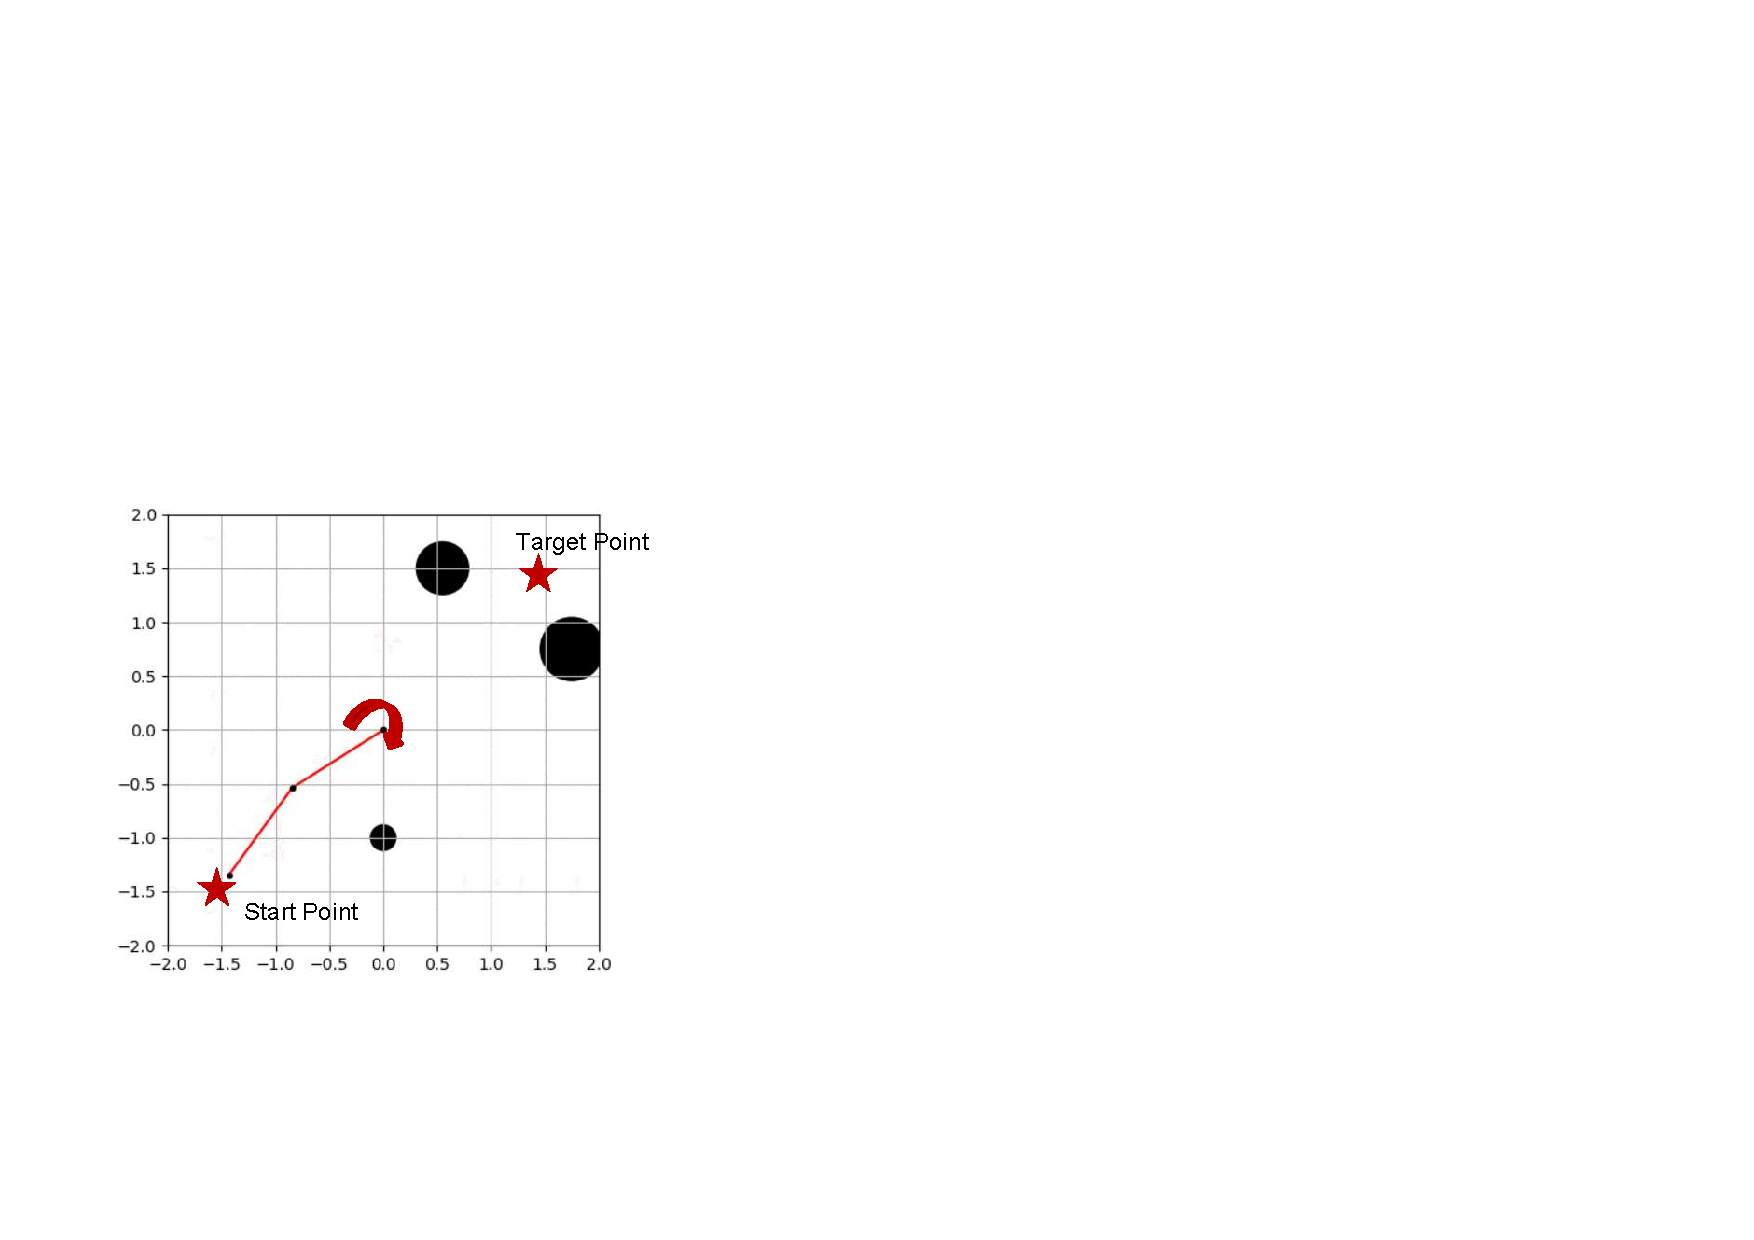
\includegraphics[width=0.5\textwidth]{Physical System Description}
}
\caption{Robotic arm finding a path to target point}
\label{Fig:Robotic arm} 
\end{center}
\end{figure}

\subsubsection{Goal Statements} \label{sec_Goal}    

\noindent Given the initial joint angles, the goal joint angles, and the obstacle locations, the goal statements are:

\begin{itemize}

\item[GS\refstepcounter{goalnum}\thegoalnum \label{GS_CollisionFreePath}:] Compute a collision-free trajectory in joint space from the start configuration to the goal configuration.

\item[GS\refstepcounter{goalnum}\thegoalnum \label{GS_OptimizePath}:] Minimize the total path length while ensuring obstacle avoidance.

\item[GS\refstepcounter{goalnum}\thegoalnum \label{GS_SmoothMotion}:] Generate a smooth and continuous motion trajectory for the robotic arm.

\item[GS\refstepcounter{goalnum}\thegoalnum \label{GS_PathSafety}:] Validate the safety of the planned path by verifying obstacle-free movement at each configuration.

\end{itemize}

\subsection{Solution Characteristics Specification}

The instance models that govern \progname{} are presented in the Instance Model Section. The necessary information to understand the meaning of the instance models and their derivation is also included, ensuring that the instance models can be verified. The solution characteristics describe the assumptions, theoretical foundations, and mathematical formulations that define the problem space and provide a basis for trajectory planning and obstacle avoidance in robotic arm motion.


\begin{figure}[H]
  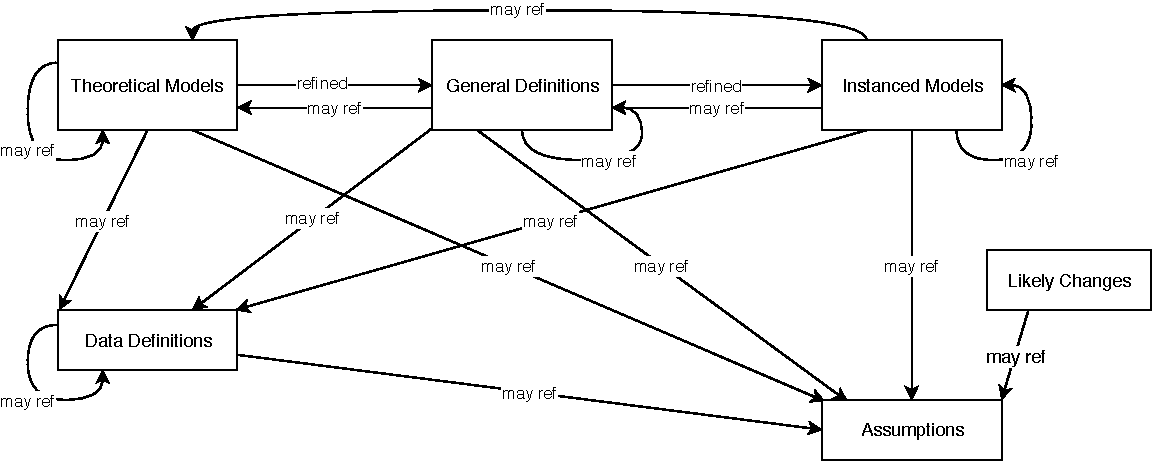
\includegraphics[scale=0.9]{RelationsBetweenTM_GD_IM_DD_A.pdf}
\end{figure}

The instance models that govern \progname{} are presented in
Subsection~\ref{sec_instance}.  The information to understand the meaning of the
instance models and their derivation is also presented, so that the instance
models can be verified.

\subsubsection{Assumptions} \label{sec_assumpt}


This section simplifies the original problem and helps in developing the
theoretical model by filling in the missing information for the physical system.
The numbers given in the square brackets refer to the theoretical model [TM],
general definition [GD], data definition [DD], instance model [IM], or likely
change [LC], in which the respective assumption is used.

\begin{itemize}

  \item[A\refstepcounter{assumpnum}\theassumpnum \label{A_KinematicMotionOnly}:] 
  The motion of the robotic arm is modeled purely kinematically, without considering the effects of dynamics such as forces, torques, or friction. (RefBy: IM:PathPlanning)

\item[A\refstepcounter{assumpnum}\theassumpnum \label{A_LinkLengthsConstant}:] 
  The lengths of all links in the robotic arm are constant and do not change during motion. (RefBy: GD:ForwardKinematics)

\item[A\refstepcounter{assumpnum}\theassumpnum \label{A_JointMotionContinuous}:] 
  The joint angles of the robotic arm vary smoothly and continuously without sudden jumps. (RefBy: IM:TrajectoryGeneration)

\item[A\refstepcounter{assumpnum}\theassumpnum \label{A_NoMechanicalDeflection}:] 
  The robotic arm links are considered rigid, meaning there is no mechanical deflection or deformation. (RefBy: GD:InverseKinematics)

\item[A\refstepcounter{assumpnum}\theassumpnum \label{A_ObstacleShapeCircular}:] 
  Obstacles in the environment are approximated as circles with predefined radii. (RefBy: IM:CollisionDetection)

\item[A\refstepcounter{assumpnum}\theassumpnum \label{A_TrajectoryDiscretized}:] 
  The planned trajectory is discretized into a series of intermediate waypoints in joint space. (RefBy: IM:TrajectoryGeneration)

\item[A\refstepcounter{assumpnum}\theassumpnum \label{A_InitialAndGoalConfigurationsKnown}:] 
  The initial joint configuration and the goal joint configuration are known before path planning begins. (RefBy: IM:PathPlanning)

\end{itemize}

\subsubsection{Theoretical Models}\label{sec_theoretical}

This section focuses on the general equations and laws that \progname{} is based
on. The theoretical models serve as fundamental principles governing the kinematic motion and path planning of the robotic arm. 

~\newline

\noindent
\deftheory
% #2 refname of theory
{TM:FWDKinematics}
% #3 label
{Forward Kinematics}
% #4 equation
{
  $\mathbf{x} = f(\mathbf{q}) = \begin{bmatrix}
  L_1 \cos(\theta_1) + L_2 \cos(\theta_1 + \theta_2) \\
  L_1 \sin(\theta_1) + L_2 \sin(\theta_1 + \theta_2)
  \end{bmatrix}$
}
% #5 description
{
  \begin{itemize}
    \item $\mathbf{q}$: Joint angles, where $\theta_1$ is the angle of the first joint and $\theta_2$ is the relative angle of the second joint.
    \item $L_1$: Length of the first link (\si{\milli\metre}).
    \item $L_2$: Length of the second link (\si{\milli\metre}).
  \end{itemize}
}
% #6 Notes
{
  This forward kinematics model assumes:
  \begin{itemize}
    \item Rigid links: The links are assumed to be perfectly rigid and do not deform under load (\aref{A_LinkLengthsConstant}).
    \item Fixed base: The base of the arm is considered stationary, located at the origin $(0, 0)$.
    \item Ideal joints: The joints rotate without friction or other physical limitations.
    \item Planar motion: The arm operates in a 2D plane, and there is no out-of-plane movement.
  \end{itemize}

  These assumptions ensure simplicity and accuracy for theoretical modeling. For real-world applications, additional factors such as joint compliance, link flexibility, and external forces may need to be considered.
}
% #7 Source
{
  \url{https://atsushisakai.github.io/PythonRobotics/modules/7_arm_navigation/planar_two_link_ik.html}
}
% #8 Referenced by
{
  \dref{ROCT}
}
% #9 Preconditions
{
None
}
% #1 derivation - not applicable by default
{}



~\newline

\subsubsection{General Definitions}\label{sec_gendef}

This section collects the laws and equations that will be used in building the instance models.

~\newline

\noindent
\begin{minipage}{\textwidth}
\renewcommand*{\arraystretch}{1.5}
\begin{tabular}{| p{\colAwidth} | p{\colBwidth}|}
\hline
\rowcolor[gray]{0.9}
Number& GD\refstepcounter{defnum}\thedefnum \label{GD_FWD_Kinematics}\\
\hline
Label &\bf Forward Kinematics of a 2D Robotic Arm \\ 
\hline
SI Units&\si{\milli\metre}\\
\hline
Equation&
\[
\begin{aligned}
    x &= L_1 \cos(\theta_1) + L_2 \cos(\theta_1 + \theta_2) \\
    y &= L_1 \sin(\theta_1) + L_2 \sin(\theta_1 + \theta_2)
\end{aligned}
\]
\\
\hline
Description & 
The forward kinematics equations describe the position of the end-effector in Cartesian coordinates given the joint angles and link lengths.
\\
& $x, y$ are the Cartesian coordinates of the end-effector (\si{\milli\metre}).\\
& $L_1, L_2$ are the lengths of the arm’s links (\si{\milli\metre}).\\
& $\theta_1, \theta_2$ are the joint angles (radians).\\
& Assumptions:
\begin{itemize}
    \item The links are rigid and have fixed lengths (\aref{A_LinkLengthsConstant}).
    \item The joints rotate freely within the plane.
    \item The base of the robotic arm is fixed.
\end{itemize}
\\
\hline
Source &--\\
\hline
% Ref.\ By & \dref{GD_Inverse_Kinematics}, \dref{IM_PathPlanning}\\
\hline
\end{tabular}
\end{minipage}\\

\subsubsection*{Detailed derivation of forward kinematics equations}
The forward kinematics of a 2D robotic arm is derived by considering the arm as a series of rigid links connected by rotational joints. The position of the end-effector is computed as follows:

\begin{enumerate}
    \item The first joint rotates by an angle $\theta_1$, positioning the second joint at:
    \[
    x_1 = L_1 \cos(\theta_1), \quad y_1 = L_1 \sin(\theta_1).
    \]
    \item The second joint rotates by an angle $\theta_2$, contributing to the final position:
    \[
    x = x_1 + L_2 \cos(\theta_1 + \theta_2), \quad y = y_1 + L_2 \sin(\theta_1 + \theta_2).
    \]
    \item Substituting $x_1$ and $y_1$ results in the final equations:
    \[
    x = L_1 \cos(\theta_1) + L_2 \cos(\theta_1 + \theta_2),
    \]
    \[
    y = L_1 \sin(\theta_1) + L_2 \sin(\theta_1 + \theta_2).
    \]
\end{enumerate}

These equations provide a direct mapping from joint space to Cartesian space, which is essential for path planning and trajectory control in robotic applications.

\subsubsection{Data Definitions}\label{sec_datadef}

This section defines and collects the essential data needed to build the instance models. The variables defined here will be used throughout the document.

\noindent
\begin{minipage}{\textwidth}
\renewcommand*{\arraystretch}{1.5}
\begin{tabular}{| p{\colAwidth} | p{\colBwidth}|}
\hline
\rowcolor[gray]{0.9}
Number & DD\refstepcounter{datadefnum}\thedatadefnum \label{DD_FWD_Kinematics}\\
\hline
Label & \bf Forward Kinematics Data Definition\\
\hline
Symbol & $\mathbf{x} = (x, y)$\\
\hline
SI Units & \si{\milli\metre}\\
\hline
Equation &
\[
\begin{aligned}
    x &= L_1 \cos(\theta_1) + L_2 \cos(\theta_1 + \theta_2) \\
    y &= L_1 \sin(\theta_1) + L_2 \sin(\theta_1 + \theta_2)
\end{aligned}
\]
\\
\hline
Description & 
Forward kinematics describes how the end-effector position in Cartesian coordinates $(x, y)$ is computed as a function of the joint angles $\theta_1, \theta_2$ and link lengths $L_1, L_2$. 

\begin{itemize}
    \item $x, y$: Cartesian coordinates of the end-effector (\si{\milli\metre}).
    \item $L_1, L_2$: Lengths of the robotic arm's links (\si{\milli\metre}).
    \item $\theta_1, \theta_2$: Joint angles (radians).
\end{itemize}

This assumes:
\begin{itemize}
    \item The robotic arm operates in a 2D plane.
    \item The links are rigid with fixed lengths (\aref{A_LinkLengthsConstant}).
    \item The base of the robotic arm is fixed at $(0,0)$.
\end{itemize}
\\
\hline
Source & Robotics textbook or relevant reference\\
\hline
Ref.\ By & \dref{GD_Inverse_Kinematics}, \dref{IM_PathPlanning}\\
\hline
\end{tabular}
\end{minipage}\\



\subsubsection{Data Types}\label{sec_datatypes}

This section defines the data types used in the robotic arm path planning (2D-RAPP) system. These types are used to specify inputs, intermediate values, and outputs in the models.

~\newline

\noindent
\begin{minipage}{\textwidth}
\renewcommand*{\arraystretch}{1.5}
\begin{tabular}{| p{\colAwidth} | p{\colBwidth}|}
  \hline
  \rowcolor[gray]{0.9}
  Type Name & Description\\
  \hline
  \texttt{Angle} & Represents joint angles of the robotic arm in radians. \\
  \hline
  \texttt{Length} & Represents physical lengths (e.g., arm links, obstacle radii) in millsmeters. \\
  \hline
  \texttt{Position} & A 2D Cartesian coordinate represented as $(x, y)$ in millsmeters. \\
  \hline
  \texttt{Velocity} & Represents joint angular velocity in radians per second. \\
  \hline
  \texttt{Acceleration} & Represents joint angular acceleration in radians per second squared. \\
  \hline
  \texttt{Trajectory} & A sequence of joint angles describing the motion plan. \\
  \hline
  \texttt{Obstacle} & A structure containing an obstacle's center position $(x, y)$ and radius. \\
  \hline
  \texttt{Boolean} & A binary value (true/false) indicating feasibility of a path. \\
  \hline
\end{tabular}
\end{minipage}\\


\subsubsection{Instance Models} \label{sec_instance}

This section transforms the problem defined in Section~\ref{Sec_pd} into one expressed in mathematical terms. It uses concrete symbols defined in Section~\ref{sec_datadef} to replace the abstract symbols in the models identified in Sections~\ref{sec_theoretical} and~\ref{sec_gendef}.

The goal statements \ref{sec_Goal} are addressed by the following instance models:

~\newline

\noindent
\deftheory
% #2 refname of theory
{IM:TrajectoryGeneration}
% #3 label
{Trajectory Generation}
% #4 equation
{
  $\mathbf{q}(t) = \text{PathPlanner}(\mathbf{q}_{\text{init}}, \mathbf{q}_{\text{goal}}, O, r)$
}
% #5 description
{
  The trajectory generation model computes a smooth, collision-free sequence of joint angles $\mathbf{q}(t)$ 
  (radians) to move the robotic arm from the initial configuration $\mathbf{q}_{\text{init}}$ to the goal 
  configuration $\mathbf{q}_{\text{goal}}$. The function $\text{PathPlanner}$ considers obstacle locations 
  $O_i$ and radii $r_i$ to avoid collisions.

  The planned trajectory satisfies the following conditions:
  \begin{itemize}
    \item The path is kinematically feasible, considering joint limits and maximum velocities.
    \item No path segment intersects any obstacle.
    \item If no valid path exists, the system returns an empty trajectory and an infeasibility warning.
  \end{itemize}
}
% #6 Notes
{
This model assumes a 2D planar manipulator with revolute joints and no external disturbances (\aref{A_NoExternalDisturbances}).
}
% #7 Source
{
  \url{https://www.robotics.org/path_planning}
}
% #8 Referenced by
{
  \rref{R_Calculate}, \rref{R_Output}
}
% #9 Preconditions
{
  The start and goal configurations must be valid joint states within the robot’s joint limits.
}
% #1 derivation - not applicable by default
{}

~\newline

\noindent
\deftheory
% #2 refname of theory
{IM:ObstacleAvoidance}
% #3 label
{Obstacle Avoidance}
% #4 equation
{
  $ \min\limits_{i} \left\| \mathbf{x}(t) - O_i \right\| \geq r_i + \epsilon, \quad \forall t $
}
% #5 description
{
  This model ensures that the robotic arm does not collide with obstacles during motion. The distance 
  between the end-effector position $\mathbf{x}(t)$ and each obstacle center $O_i$ must always be 
  greater than the obstacle radius $r_i$ plus a safety margin $\epsilon$.

  This condition is checked at every time step of the planned trajectory. If violated, a new trajectory 
  is generated, or an infeasibility warning is returned.
}
% #6 Notes
{
  This model assumes that obstacle positions remain static during execution (\aref{A_StaticObstacles}).
}
% #7 Source
{
  \url{https://www.robotics.org/collision_avoidance}
}
% #8 Referenced by
{
  \rref{R_Calculate}, \rref{R_VerifyOutput}
}
% #9 Preconditions
{
  The obstacle positions and radii must be known before trajectory planning.
}
% #1 derivation - not applicable by default
{}


~\newline


%~\newline

\subsubsection*{Derivation of Trajectory Generation (IM:TrajectoryGeneration)}

The trajectory generation model is derived from forward kinematics and inverse kinematics principles. 

\begin{enumerate}
    \item \textbf{Forward Kinematics:} The position of the end-effector $\mathbf{x}(t)$ is determined using:
    \[
    x = L_1 \cos(\theta_1) + L_2 \cos(\theta_1 + \theta_2)
    \]
    \[
    y = L_1 \sin(\theta_1) + L_2 \sin(\theta_1 + \theta_2)
    \]
    This establishes the mapping from joint space $\mathbf{q}(t)$ to Cartesian space.

    \item \textbf{Inverse Kinematics:} Given a desired goal position $\mathbf{x}_{\text{goal}} = (x_g, y_g)$, we solve for the required joint angles:
    \[
    \theta_2 = \cos^{-1} \left(\frac{x_g^2 + y_g^2 - L_1^2 - L_2^2}{2 L_1 L_2} \right)
    \]
    \[
    \theta_1 = \tan^{-1} \left(\frac{y_g}{x_g} \right) - \tan^{-1} \left(\frac{L_2 \sin \theta_2}{L_1 + L_2 \cos \theta_2} \right)
    \]
    This establishes the mapping from Cartesian space to joint space.

    \item \textbf{Path Planning:} A trajectory $\mathbf{q}(t)$ is generated using an interpolation method such as:
    \begin{itemize}
        \item Linear interpolation (for simple movements).
        \item Polynomial interpolation (e.g., cubic splines) for smooth acceleration profiles.
        \item Graph-based search algorithms (e.g., A* on a discretized joint space).
    \end{itemize}

    \item \textbf{Collision Avoidance:} Each planned trajectory segment is verified against obstacles using:
    \[
    \min\limits_{i} \left\| \mathbf{x}(t) - O_i \right\| \geq r_i + \epsilon, \quad \forall t
    \]
    If this constraint is violated, a new path is computed, or an infeasibility warning is returned.
\end{enumerate}

The derivation combines these principles to ensure a feasible, collision-free trajectory for the robotic arm.

\subsubsection*{Derivation of Obstacle Avoidance (IM:ObstacleAvoidance)}

Obstacle avoidance is derived from the Euclidean distance constraint:

\begin{enumerate}
    \item \textbf{Obstacle Representation:} Obstacles are modeled as circles with centers $O_i = (O_{i_x}, O_{i_y})$ and radii $r_i$.

    \item \textbf{Collision Condition:} A collision occurs if:
    \[
    \left\| \mathbf{x}(t) - O_i \right\| < r_i
    \]
    where $\mathbf{x}(t)$ is the end-effector position.

    \item \textbf{Safe Clearance Constraint:} To avoid collisions, the trajectory must satisfy:
    \[
    \left\| \mathbf{x}(t) - O_i \right\| \geq r_i + \epsilon, \quad \forall t
    \]
    where $\epsilon$ is a safety margin.

    \item \textbf{Validation:} Each trajectory segment is checked at discrete time steps. If a collision is detected, the path planner reattempts a new trajectory.
\end{enumerate}

This derivation ensures that the robotic arm follows a valid path while maintaining a safe distance from obstacles.


\subsubsection{Input Data Constraints} \label{sec_DataConstraints}    

Table~\ref{TblInputVar} shows the data constraints on the input variables. The column for physical constraints gives the physical limitations on the range of values that can be taken by the variable. The column for software constraints restricts the range of inputs to reasonable values. These software constraints will be helpful in the design stage for selecting suitable algorithms. The constraints are conservative to give users flexibility in experimenting with unusual situations. The column of typical values provides a reference for common scenarios. The uncertainty column estimates the confidence with which the physical quantities can be measured. This information is useful for uncertainty quantification exercises.

The specification parameters in Table~\ref{TblInputVar} are listed in Table~\ref{TblSpecParams}.

\begin{table}[!h]
  \caption{Input Variables for 2D-RAPP} \label{TblInputVar}
  \renewcommand{\arraystretch}{1.2}
\noindent \begin{longtable*}{l l l l c} 
  \toprule
  \textbf{Var} & \textbf{Physical Constraints} & \textbf{Software Constraints} &
                             \textbf{Typical Value} & \textbf{Uncertainty}\\
  \midrule 
  $L_1, L_2$ & $L_i > 0$ & $L_{\text{min}} \leq L_i \leq L_{\text{max}}$ & 1.0 \si[per-mode=symbol] {\metre} & 5\%
  \\
  $\theta_1, \theta_2$ & $-\pi \leq \theta_i \leq \pi$ & $-\pi \leq \theta_i \leq \pi$ & 0 \si[per-mode=symbol]{\radian} & 1\%
  \\
  $x_{\text{goal}}, y_{\text{goal}}$ & Defined workspace bounds & Within reachable workspace & (1.5, 1.5) \si[per-mode=symbol]{\metre} & 10\%
  \\
  $r_{\text{obs}}$ & $r_{\text{obs}} > 0$ & $r_{\text{obs}} \leq r_{\text{max}}$ & 0.3 \si[per-mode=symbol]{\metre} & 5\%
  \\
  $(x_{\text{obs}}, y_{\text{obs}})$ & Within workspace bounds & Within workspace bounds & (0.5, 0.5) \si[per-mode=symbol]{\metre} & 10\%
  \\
  \bottomrule
\end{longtable*}
\end{table}

\noindent 
\begin{description}
\item[(*)] $\theta_1, \theta_2$ are the joint angles of the robotic arm.
\item[(*)] $L_1, L_2$ are the lengths of the arm segments.
\item[(*)] $x_{\text{goal}}, y_{\text{goal}}$ define the Cartesian coordinates of the target.
\item[(*)] $(x_{\text{obs}}, y_{\text{obs}})$ and $r_{\text{obs}}$ define the position and size of obstacles.
\end{description}

\begin{table}[!h]
\caption{Specification Parameter Values for 2D-RAPP} \label{TblSpecParams}
\renewcommand{\arraystretch}{1.2}
\noindent \begin{longtable*}{l l} 
  \toprule
  \textbf{Var} & \textbf{Value} \\
  \midrule 
  $L_\text{min}$ & 0.1 \si{\metre}\\
  $L_\text{max}$ & 2.0 \si{\metre}\\
  $r_{\text{max}}$ & 0.5 \si{\metre}\\
  \bottomrule
\end{longtable*}
\end{table}


\subsubsection{Properties of a Correct Solution} \label{sec_CorrectSolution}

\noindent
A correct solution must exhibit the following properties to ensure robustness and feasibility in robotic arm path planning:

\begin{itemize}
    \item The generated trajectory must be \textbf{collision-free}, ensuring that the robotic arm does not intersect any obstacles.
    \item The computed joint angles (\(\theta_1, \theta_2\)) must respect the physical limits of the robotic arm.
    \item The path must be \textbf{kinematically feasible}, meaning it can be executed smoothly by the robotic system.
    \item If the target position is unreachable due to obstacles or arm constraints, the system must return an empty trajectory and notify the user.
\end{itemize}

\noindent
Additionally, output values must adhere to known physical constraints, summarized in Table~\ref{TblOutputVar}.

\begin{table}[!h]
\caption{Output Variables and Physical Constraints} \label{TblOutputVar}
\renewcommand{\arraystretch}{1.2}
\noindent \begin{longtable*}{l l} 
  \toprule
  \textbf{Var} & \textbf{Physical Constraints} \\
  \midrule 
  $\theta_1, \theta_2$ & $-\pi \leq \theta_1, \theta_2 \leq \pi$ (Joint limits) \\
  $(x, y)$ & Within reachable workspace of arm \\
  $\mathbf{q}_{\text{path}}$ & Must be collision-free with obstacles \\
  $\mathbf{x}_{\text{goal}}$ & If unreachable, return empty trajectory \\
  \bottomrule
\end{longtable*}
\end{table}

\noindent
These constraints ensure that the computed motion plan is valid, achievable, and safe for execution by the robotic arm.


\section{Requirements}

This section provides the functional requirements, the business tasks that the
software is expected to complete, and the nonfunctional requirements, the
qualities that the software is expected to exhibit.

\subsection{Functional Requirements}

\noindent \begin{itemize}

  \item[R\refstepcounter{reqnum}\thereqnum \label{R_Inputs}:]  
    The system shall accept the following inputs from the user:
    \begin{itemize}
      \item Initial joint angles \( q_{\text{init}} = (\theta_1, \theta_2) \) in radians.
      \item Goal position \( (x_{\text{goal}}, y_{\text{goal}}) \) in Cartesian coordinates (\si{\milli\metre}).
      \item Obstacle positions \( O_i = (x_i, y_i) \) and radii \( r_i \) (\si{\milli\metre}).
      \item Link lengths \( L_1, L_2 \) of the robotic arm (\si{\milli\metre}).
    \end{itemize}
  
  \item[R\refstepcounter{reqnum}\thereqnum \label{R_OutputInputs}:]  
    The system shall echo all input values to ensure correctness before computation.
  
  \item[R\refstepcounter{reqnum}\thereqnum \label{R_Calculate}:]  
    The system shall perform the following calculations:
    \begin{itemize}
      \item Compute the forward kinematics to determine the end-effector position.
      \item Determine the collision-free path from \( q_{\text{init}} \) to the goal using A* search.
      \item Generate the sequence of intermediate joint configurations \( q(t) \) for smooth motion.
    \end{itemize}
  
  \item[R\refstepcounter{reqnum}\thereqnum \label{R_VerifyOutput}:]  
    The system shall verify that:
    \begin{itemize}
      \item The computed path avoids all obstacles.
      \item The final joint configuration corresponds to the given goal position.
      \item The output trajectory is continuous and feasible for the robotic arm.
    \end{itemize}
  
  \item[R\refstepcounter{reqnum}\thereqnum \label{R_Output}:]  
    The system shall output the following:
    \begin{itemize}
      \item The computed path in joint space, represented as a sequence of joint angles \( q(t) \).
      \item The Cartesian positions of the end-effector throughout the motion.
      \item A visualization of the planned motion with the robotic arm and obstacles.
    \end{itemize}
  
  \end{itemize}
  
  \subsection{Nonfunctional Requirements}

  This section defines the nonfunctional requirements that specify the qualities and characteristics the software should exhibit.
  
  \noindent \begin{itemize}
  
  \item[NFR\refstepcounter{nfrnum}\thenfrnum \label{NFR_Accuracy}:]  
    \textbf{Accuracy} \\
    The system shall compute the robotic arm trajectory with an accuracy sufficient for motion planning in a dynamic environment. The precision of the joint angles shall be within \(0.01\) radians, and the calculated Cartesian positions of the end-effector shall have an error margin within \(0.1\) cm. The accuracy shall be validated through simulation and empirical testing.
  
  \item[NFR\refstepcounter{nfrnum}\thenfrnum \label{NFR_Maintainability}:]  
    \textbf{Maintainability} \\
    The effort required to make likely modifications to the software (such as adjusting the planning algorithm or adding new constraints) shall be at most \(10\%\) of the original development time, assuming the same development resources are available. Code modularization and documentation will facilitate future modifications.

  \item[NFR\refstepcounter{nfrnum}\thenfrnum \label{NFR_Verifiability}:]  
    \textbf{Verifiability} \\
    The correctness of the system shall be tested with a complete verification and validation (V\&V) plan. The outputs shall be compared against theoretical models and experimental data.
  
  \item[NFR\refstepcounter{nfrnum}\thenfrnum \label{NFR_Understandability}:]  
    \textbf{Understandability} \\
    The software shall follow a modular architecture with clear documentation, including a module guide and interface specification. Each function and class shall have inline comments explaining its purpose and usage.a
  
  \item[NFR\refstepcounter{nfrnum}\thenfrnum \label{NFR_Reusability}:]  
    \textbf{Reusability} \\
    The system shall be designed with reusability in mind, allowing for easy adaptation to different robotic configurations. The kinematic and planning modules shall be abstracted so they can be reused in other robotic applications.
  
  \end{itemize}
  

  \subsection{Rationale}

  This section provides justifications for the decisions made in the documentation, including scope choices, modeling approaches, assumptions, and typical values.
  
  \noindent \begin{itemize}
  
  \item \textbf{Scope Decisions:}  
  The scope is limited to 2D kinematic motion planning for a two-link robotic arm. This choice simplifies computations by avoiding the complexities of dynamic control and multi-degree-of-freedom motion. The system focuses on trajectory planning and collision avoidance, which are critical for robotic applications in structured environments.
  
  \item \textbf{Modeling Decisions:}  
  The system models the robotic arm using forward kinematics and inverse kinematics equations. The choice of the A* algorithm for trajectory planning ensures optimal pathfinding in discrete joint space. A toroidal occupancy grid is used to handle the periodic nature of joint angles while maintaining computational efficiency.
  
  \item \textbf{Assumptions:}  
  Several assumptions were made to reduce computational complexity and improve efficiency:
    \begin{itemize}
      \item The robotic arm consists of two rigid links with fixed lengths (\aref{A_LinkLengthsConstant}).
      \item The motion occurs strictly in a 2D plane, ignoring dynamic effects such as inertia and external forces.
      \item The joint angles are constrained within \([- \pi, \pi]\) to ensure practical movement constraints.
    \end{itemize}
  
  \item \textbf{Typical Values:}  
  The choice of typical values for input parameters is based on real-world robotic systems:
    \begin{itemize}
      \item Link lengths (\si{\milli\metre}): $L_1 = 50$, $L_2 = 40$ 
      \item Joint angle range (\si{\radian}): $[-\pi, \pi]$
      \item Obstacle radii (\si{\milli\metre}): $r_i \in [5, 15]$ 
    \end{itemize}
    These values ensure a balance between computational efficiency and practical usability.
  
  \end{itemize}
  


  \section{Likely Changes}    

  \noindent \begin{itemize}
  
  \item[LC\refstepcounter{lcnum}\thelcnum\label{LC_GridResolution}:]  
  The resolution of the discrete grid used for A* search may need to be adjusted for better accuracy or computational efficiency. A finer grid provides more precise motion planning but increases computation time. (\aref{A_TrajectoryDiscretized})
  
  \item[LC\refstepcounter{lcnum}\thelcnum\label{LC_ObstacleShapes}:]  
  Currently, obstacles are modeled as circles for simplicity. Future iterations may need to support arbitrary polygonal obstacles to better reflect real-world scenarios. (\aref{A_ObstacleShapeCircular})
  
  \item[LC\refstepcounter{lcnum}\thelcnum\label{LC_PathPlanningAlgorithm}:]  
  The path-planning algorithm may need to be changed. Alternatives such as RRT (Rapidly-exploring Random Tree) or D* Lite might be required for more complex environments or real-time applications. 
  
  \item[LC\refstepcounter{lcnum}\thelcnum\label{LC_Kinematics}:]  
  If the system is extended to 3D, the forward kinematics equations will need to be updated to account for additional degrees of freedom. 
  
  \item[LC\refstepcounter{lcnum}\thelcnum\label{LC_JointLimits}:]  
  The current joint angle limits assume a symmetric range of motion. Some robotic arms have mechanical constraints that may require asymmetric limits, which would need to be accounted for in the calculations.
  
  \end{itemize}

  \section{Unlikely Changes}    

  \noindent \begin{itemize}
  
  \item[LC\refstepcounter{lcnum}\thelcnum\label{LC_FixedLinkLengths}:]  
  The link lengths of the robotic arm are assumed to be fixed. Future versions are not expected to support variable-length arms or telescopic links. (\aref{A_LinkLengthsConstant})
  
  
  \item[LC\refstepcounter{lcnum}\thelcnum\label{LC_NoDynamics}:]  
  The system is based purely on kinematics and does not consider dynamics (forces, torques, or inertia). It is unlikely that dynamics will be incorporated in this version. (\aref{A_KinematicMotionOnly})
  
  \item[LC\refstepcounter{lcnum}\thelcnum\label{LC_FixedCollisionDetection}:]  
  The collision detection method assumes static obstacles. It is unlikely that dynamic obstacles (moving objects) will be introduced in this implementation. (\aref{A_ObstacleShapeCircular})
  
  \end{itemize}
  

\section{Traceability Matrices and Graphs}

The purpose of the traceability matrices is to provide easy references on what
has to be additionally modified if a certain component is changed.  Every time a
component is changed, the items in the column of that component that are marked
with an ``X'' may have to be modified as well.  Table~\ref{Table:trace} shows the
dependencies of theoretical models, general definitions, data definitions, and
instance models with each other. Table~\ref{Table:R_trace} shows the
dependencies of instance models, requirements, and data constraints on each
other. Table~\ref{Table:A_trace} shows the dependencies of theoretical models,
general definitions, data definitions, instance models, and likely changes on
the assumptions.


\afterpage{
\begin{landscape}
  \begin{table}[h!]
    \centering
\begin{tabular}{|c|c|c|c|c|c|c|c|c|c|c|c|c|c|c|c|c|c|c|c|}
\hline
	& \aref{A_OnlyThermalEnergy}& \aref{A_hcoeff}& \aref{A_mixed}& \aref{A_tpcm}& \aref{A_const_density}& \aref{A_const_C}& \aref{A_Newt_coil}& \aref{A_tcoil}& \aref{A_tlcoil}& \aref{A_Newt_pcm}& \aref{A_charge}& \aref{A_InitTemp}& \aref{A_OpRangePCM}& \aref{A_OpRange}& \aref{A_htank}& \aref{A_int_heat}& \aref{A_vpcm}& \aref{A_PCM_state}& \aref{A_Pressure} \\
\hline
    \iref{IM_CollisionAvoidance} &  &  &  & X & X & X \\
    \hline
    \end{tabular}
    \end{table}
    
\end{landscape}
}

\begin{table}[h!]
\centering
\begin{tabular}{|c|c|c|c|c|c|c|c|c|c|c|c|c|c|c|c|c|c|c|c|c|c|c|c|}
\hline        
	& \tref{T_COE}& \tref{T_SHE}& \tref{T_LHE}& \dref{NL}& \dref{ROCT} & \ddref{FluxCoil}& \ddref{FluxPCM} & \ddref{D_HOF}& \ddref{D_MF}& \iref{ewat}& \iref{epcm}& \iref{I_HWAT}& \iref{I_HPCM} \\
\hline
\tref{T_COE}     & & & & & & & & & & & & & \\ \hline
\tref{T_SHE}     & & & X& & & & & & & & & & \\ \hline
\tref{T_LHE}     & & & & & & & & & & & & & \\ \hline
\dref{NL}        & & & & & & & & & & & & & \\ \hline
\dref{ROCT}      & X& & & & & & & & & & & & \\ \hline
\ddref{FluxCoil} & & & & X& & & & & & & & & \\ \hline
\ddref{FluxPCM}  & & & & X& & & & & & & & & \\ \hline
\ddref{D_HOF}    & & & & & & & & & & & & & \\ \hline
\ddref{D_MF}     & & & & & & & & X& & & & & \\ \hline
\iref{ewat}      & & & & & X& X& X& & & & X& & \\ \hline
\iref{epcm}      & & & & & X& & X& & X& X& & & X \\ \hline
\iref{I_HWAT}    & & X& & & & & & & & & & & \\ \hline
\iref{I_HPCM}    & & X& X& & & & X& X& X& & X& & \\
\hline
\end{tabular}
\caption{Traceability Matrix Showing the Connections Between Items of Different Sections}
\label{Table:trace}
\end{table}

\begin{table}[h!]
\centering
\begin{tabular}{|c|c|c|c|c|c|c|c|}
\hline
	& \iref{ewat}& \iref{epcm}& \iref{I_HWAT}& \iref{I_HPCM}& \ref{sec_DataConstraints}& \rref{R_RawInputs}& \rref{R_MassInputs} \\
\hline
\iref{ewat}            & & X& & & & X& X \\ \hline
\iref{epcm}            & X& & & X& & X& X \\ \hline
\iref{I_HWAT}          & & & & & & X& X \\ \hline
\iref{I_HPCM}          & & X& & & & X& X \\ \hline
\rref{R_RawInputs}     & & & & & & & \\ \hline
\rref{R_MassInputs}    & & & & & & X& \\ \hline
\rref{R_CheckInputs}   & & & & & X& & \\ \hline
\rref{R_OutputInputs}  & X& X& & & & X& X \\ \hline
\rref{R_TempWater}     & X& & & & & & \\ \hline 
\rref{R_TempPCM}       & & X& & & & & \\ \hline
\rref{R_EnergyWater}   & & & X& & & & \\ \hline
\rref{R_EnergyPCM}     & & & & X& & & \\ \hline
\rref{R_VerifyOutput}  & & & X& X& & & \\ \hline
\rref{R_timeMeltBegin} & & X& & & & & \\ \hline
\rref{R_timeMeltEnd}   & & X& & & & & \\ 
\hline
\end{tabular}
\caption{Traceability Matrix Showing the Connections Between Requirements and Instance Models}
\label{Table:R_trace}
\end{table}

The purpose of the traceability graphs is also to provide easy references on
what has to be additionally modified if a certain component is changed.  The
arrows in the graphs represent dependencies. The component at the tail of an
arrow is depended on by the component at the head of that arrow. Therefore, if a
component is changed, the components that it points to should also be
changed. Figure~\ref{Fig_ATrace} shows the dependencies of theoretical models,
general definitions, data definitions, instance models, likely changes, and
assumptions on each other. Figure~\ref{Fig_RTrace} shows the dependencies of
instance models, requirements, and data constraints on each other.



\section{Development Plan}

The development of \progname{} will be structured into multiple phases, ensuring a modular and iterative approach. The implementation will prioritize core functionalities essential for the robotic arm's motion planning, followed by enhancements for efficiency and usability.

\subsection{Phase 1: Core Functionalities}
\begin{itemize}
    \item[R\ref{R_Inputs}:] Implement user input handling for joint angles, goal position, and obstacles.
    \item[R\ref{R_Calculate}:] Develop forward kinematics calculations to determine the end-effector position from joint angles.
    \item[R\ref{R_Output}:] Display the calculated position of the end-effector.
    \item[R\ref{R_VerifyOutput}:] Verify the correctness of kinematic calculations.
\end{itemize}

\subsection{Phase 2: Path Planning}
\begin{itemize}
    \item[R\ref{R_Calculate}:] Implement inverse kinematics to compute joint angles for a given target position.
    \item[R\ref{R_Calculate}:] Integrate A* search algorithm for path planning in joint space.
    \item[R\ref{R_VerifyOutput}:] Ensure path validity by checking for obstacle collisions.
\end{itemize}

\subsection{Phase 3: Optimization and Usability Enhancements}
\begin{itemize}
    \item[NFR\ref{NFR_Accuracy}:] Improve accuracy of kinematic computations.
    \item[NFR\ref{NFR_Maintainability}:] Ensure modularity in code for easy extension.
\end{itemize}

\section{Values of Auxiliary Constants}

The following table defines symbolic constants introduced in the document for maintainability and ease of modification.

\begin{table}[h!]
\centering
\begin{tabular}{|c|c|c|}
\hline
\textbf{Symbol} & \textbf{Description} & \textbf{Value} \\
\hline
$L_1$ & Length of first arm link (\si{\milli\metre}) & 50 \\
$L_2$ & Length of second arm link (\si{\milli\metre}) & 40 \\
$\theta_{\min}$ & Minimum joint angle (\si{\degree}) & $-180$ \\
$\theta_{\max}$ & Maximum joint angle (\si{\degree}) & $180$ \\
$\Delta q$ & Discretization step for A* search (radians) & $0.1$ \\
$\text{FRACTION}$ & Fraction of original development time for maintainability & $0.1$ \\
\hline
\end{tabular}
\caption{Values of Auxiliary Constants}
\label{Table:AuxiliaryConstants}
\end{table}

\newpage

\bibliographystyle {plainnat}
\bibliography {../../refs/References}

\newpage

\newpage{}
\section*{Appendix --- Reflection}

\wss{Not required for CAS 741}

The information in this section will be used to evaluate the team members on the
graduate attribute of Lifelong Learning.  
The purpose of reflection questions is to give you a chance to assess your own
learning and that of your group as a whole, and to find ways to improve in the
future. Reflection is an important part of the learning process.  Reflection is
also an essential component of a successful software development process.  

Reflections are most interesting and useful when they're honest, even if the
stories they tell are imperfect. You will be marked based on your depth of
thought and analysis, and not based on the content of the reflections
themselves. Thus, for full marks we encourage you to answer openly and honestly
and to avoid simply writing ``what you think the evaluator wants to hear.''

Please answer the following questions.  Some questions can be answered on the
team level, but where appropriate, each team member should write their own
response:


\begin{enumerate}
  \item What went well while writing this deliverable? 
  \item What pain points did you experience during this deliverable, and how did
  you resolve them?
  \item How many of your requirements were inspired by speaking to your
  client(s) or their proxies (e.g. your peers, stakeholders, potential users)?
  \item Which of the courses you have taken, or are currently taking, will help
  your team to be successful with your capstone project.
  \item What knowledge and skills will the team collectively need to acquire to
  successfully complete this capstone project?  Examples of possible knowledge
  to acquire include domain specific knowledge from the domain of your
  application, or software engineering knowledge, mechatronics knowledge or
  computer science knowledge.  Skills may be related to technology, or writing,
  or presentation, or team management, etc.  You should look to identify at
  least one item for each team member.
  \item For each of the knowledge areas and skills identified in the previous
  question, what are at least two approaches to acquiring the knowledge or
  mastering the skill?  Of the identified approaches, which will each team
  member pursue, and why did they make this choice?
\end{enumerate}

\end{document}